\documentclass[tikz,border=12pt]{standalone}
\usepackage[T1]{fontenc}
\usepackage{mathpazo}
\usepackage{amsmath,amssymb}
\usetikzlibrary{arrows.meta, positioning, calc, fit, decorations.pathreplacing}

\definecolor{stblue}{HTML}{7B97AD}
\definecolor{rwgold}{HTML}{B8995E}
\definecolor{sage}{HTML}{7A9A7E}
\definecolor{dkbrown}{HTML}{3D3530}
\definecolor{wmgray}{HTML}{7B7067}
\definecolor{cream}{HTML}{F9F6F0}
\definecolor{border}{HTML}{D4C9B8}
\definecolor{terracotta}{HTML}{C47A6A}
\definecolor{lavender}{HTML}{907EA0}

\begin{document}
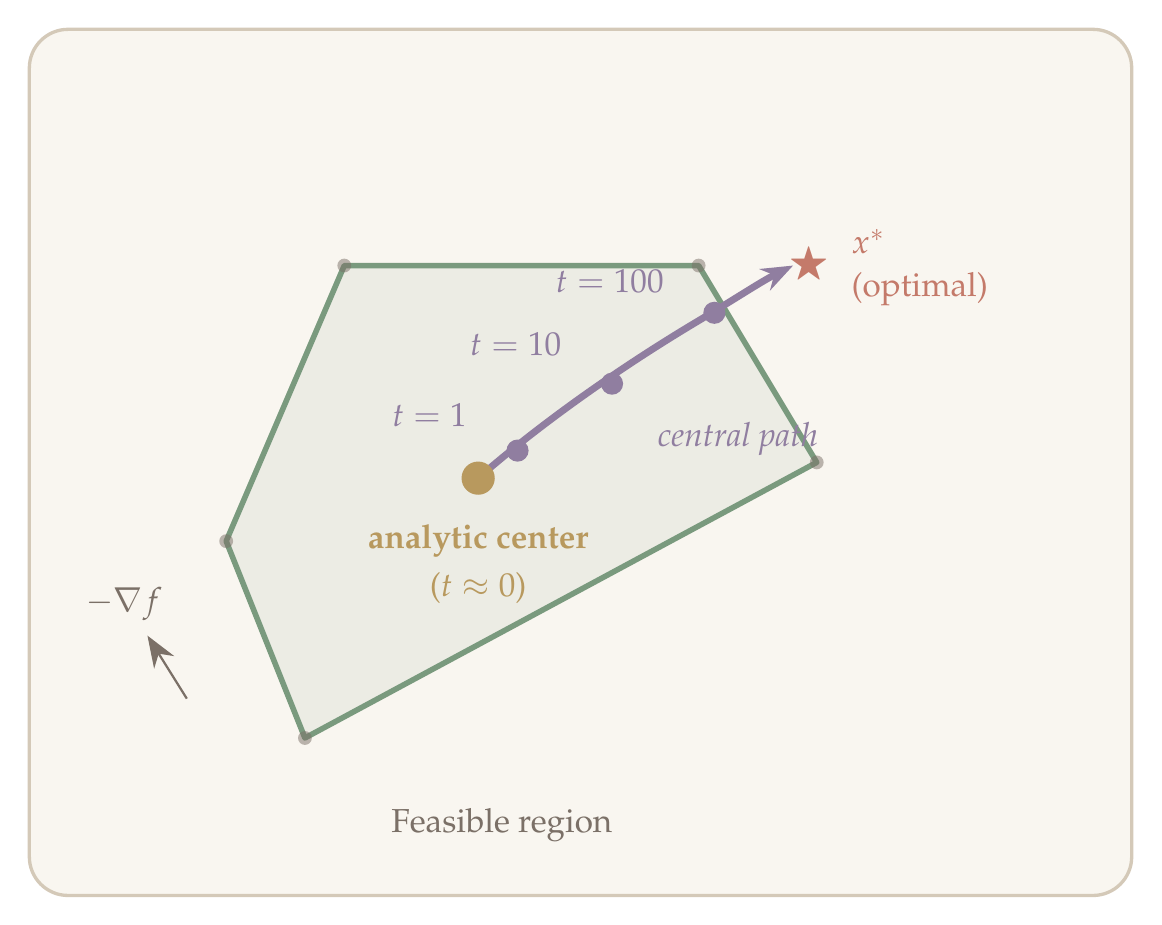
\begin{tikzpicture}[>={Stealth[length=4mm, width=3mm]}, line width=1.5pt]

% Background
\fill[cream, rounded corners=14pt] (-1.5,-1.5) rectangle (12.5,9.5);
\draw[border, line width=1.2pt, rounded corners=14pt] (-1.5,-1.5) rectangle (12.5,9.5);

% Pentagon feasible region
\fill[sage, opacity=0.10]
  (2.0,0.5) -- (1.0,3.0) -- (2.5,6.5) -- (7.0,6.5) -- (8.5,4.0) -- cycle;
\draw[sage, line width=2pt, line join=round]
  (2.0,0.5) -- (1.0,3.0) -- (2.5,6.5) -- (7.0,6.5) -- (8.5,4.0) -- cycle;
\node[text=wmgray, font=\large] at (4.5,-0.6) {Feasible region};

% Central path
\draw[lavender, line width=2.5pt, rounded corners=2pt, ->]
  (4.2,3.8) .. controls (5.0,4.5) and (6.0,5.2) .. (7.0,5.8)
  .. controls (7.5,6.1) and (7.8,6.3) .. (8.2,6.5);

% Analytic center
\fill[rwgold] (4.2,3.8) circle (6pt);
\node[text=rwgold, font=\large\bfseries] at (4.2,3.0) {analytic center};
\node[text=rwgold, font=\large] at (4.2,2.4) {($t \approx 0$)};

% Points along the path
% t=1
\fill[lavender] (4.7,4.15) circle (4pt);
\node[text=lavender, font=\large, anchor=east] at (4.2,4.6) {$t = 1$};

% t=10
\fill[lavender] (5.9,5.0) circle (4pt);
\node[text=lavender, font=\large, anchor=east] at (5.4,5.5) {$t = 10$};

% t=100
\fill[lavender] (7.2,5.9) circle (4pt);
\node[text=lavender, font=\large, anchor=east] at (6.7,6.3) {$t = 100$};

% Optimal vertex
\node[text=terracotta, font=\Large\bfseries, inner sep=0pt] at (8.4,6.5) {$\bigstar$};
\node[text=terracotta, font=\large\bfseries, anchor=west] at (8.8,6.8) {$x^*$};
\node[text=terracotta, font=\large, anchor=west] at (8.8,6.2) {(optimal)};

% Vertex markers (faint)
\foreach \x/\y in {2.0/0.5, 1.0/3.0, 2.5/6.5, 7.0/6.5, 8.5/4.0} {
  \fill[wmgray, opacity=0.5] (\x,\y) circle (2.5pt);
}

% Central path label
\node[text=lavender, font=\large\itshape] at (7.5,4.3) {central path};

% Objective direction indicator
\draw[wmgray, ->, line width=0.8pt] (0.5,1.0) -- (0.0,1.8);
\node[text=wmgray, font=\large] at (-0.3,2.2) {$-\nabla f$};

\end{tikzpicture}
\end{document}
